\documentclass[fontsize=12pt]{scrartcl}
\usepackage[margin=0.5in, a4paper]{geometry}
\usepackage{tikz}
\usepackage{amsmath}
\usepackage{pgfplots}
\usepackage{siunitx}
\usetikzlibrary{calc,patterns,angles,quotes}
\begin{document}
Write in the form $a\mathbf{i}+b\mathbf{j}$:
\newline
\newline
\begin{tabular}{p{9cm}p{9cm}}
a) 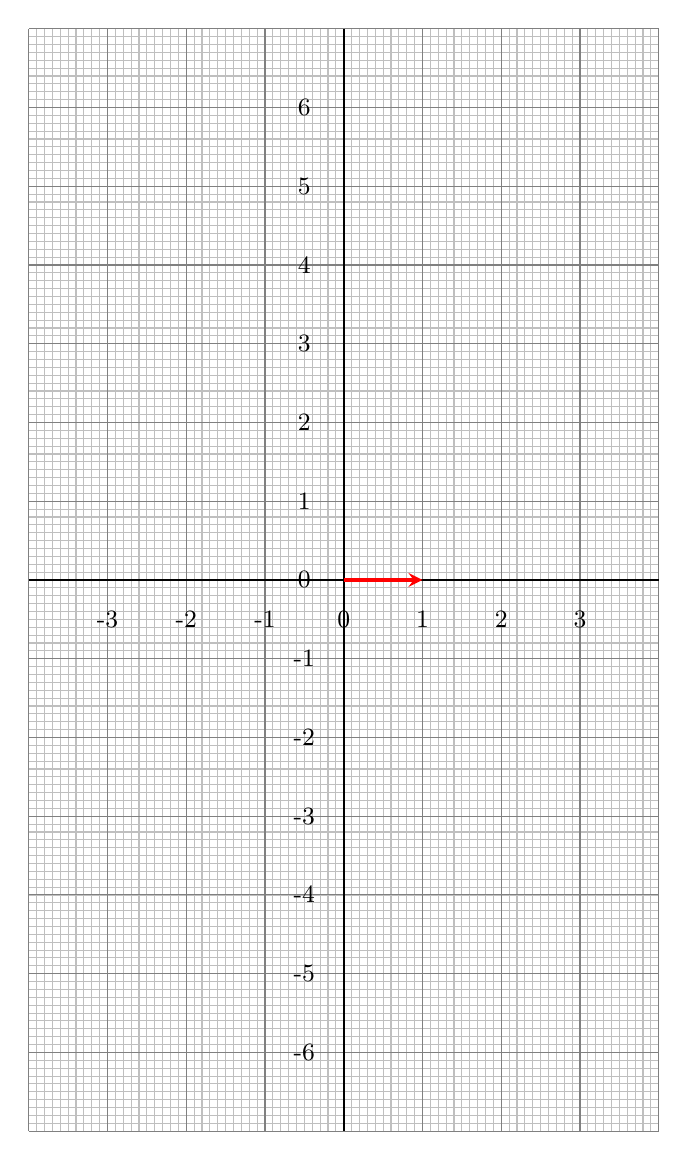
\begin{tikzpicture}
\draw[thin, step=0.1cm,color=lightgray] (-4,-7) grid (4,7);
\draw[thin, step=1cm,color=gray] (-4,-7) grid (4,7);
\draw[thick] (-4,0)--(4,0);
\draw[thick] (0,7)--(0,-7);
\foreach \x in {-3,...,3}{
  \node at (\x,-0.5)  {\small{\x}};
}
\foreach \y in {-6,...,6}{
  \node at (-0.5,\y)  {\small{\y}};
}
\draw [very thick, red, -stealth] (0,0)--(1,0);
\end{tikzpicture}
&b) 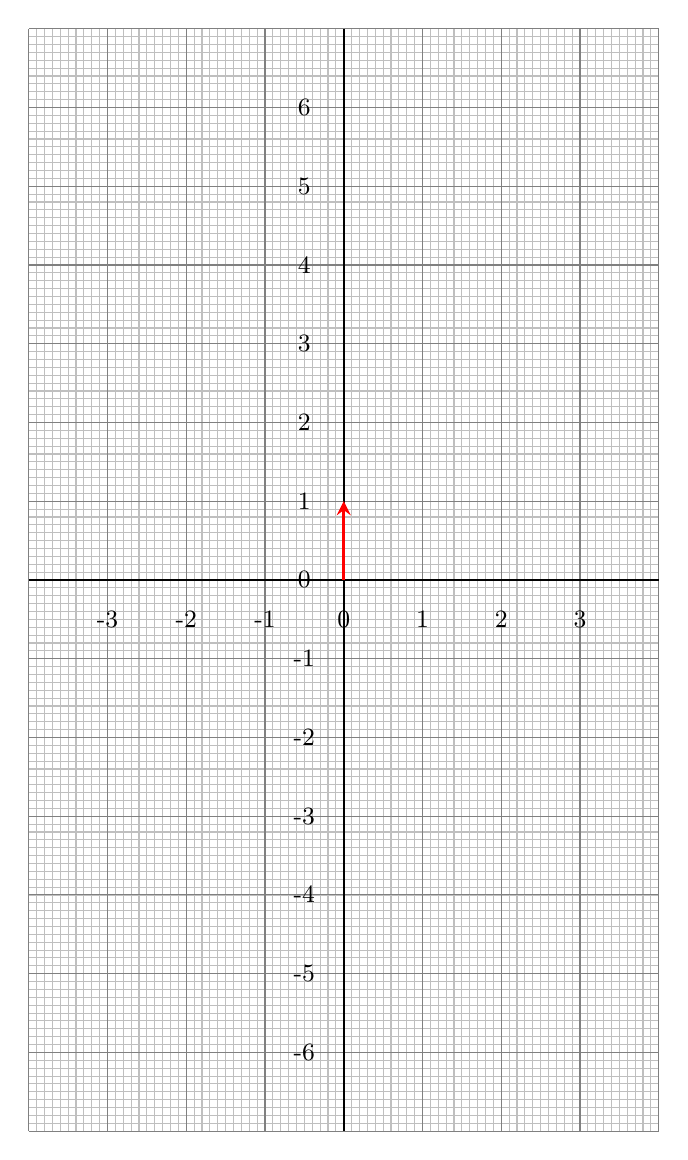
\begin{tikzpicture}
\draw[thin, step=0.1cm,color=lightgray] (-4,-7) grid (4,7);
\draw[thin, step=1cm,color=gray] (-4,-7) grid (4,7);
\draw[thick] (-4,0)--(4,0);
\draw[thick] (0,7)--(0,-7);
\foreach \x in {-3,...,3}{
  \node at (\x,-0.5)  {\small{\x}};
}
\foreach \y in {-6,...,6}{
  \node at (-0.5,\y)  {\small{\y}};
}
\draw [very thick, red, -stealth] (0,0)--(0,1);
\end{tikzpicture}
\\
\end{tabular}
\newpage
Write in the form $a\mathbf{i}+b\mathbf{j}$:
\newline
\newline
\begin{tabular}{p{9cm}p{9cm}}
a) 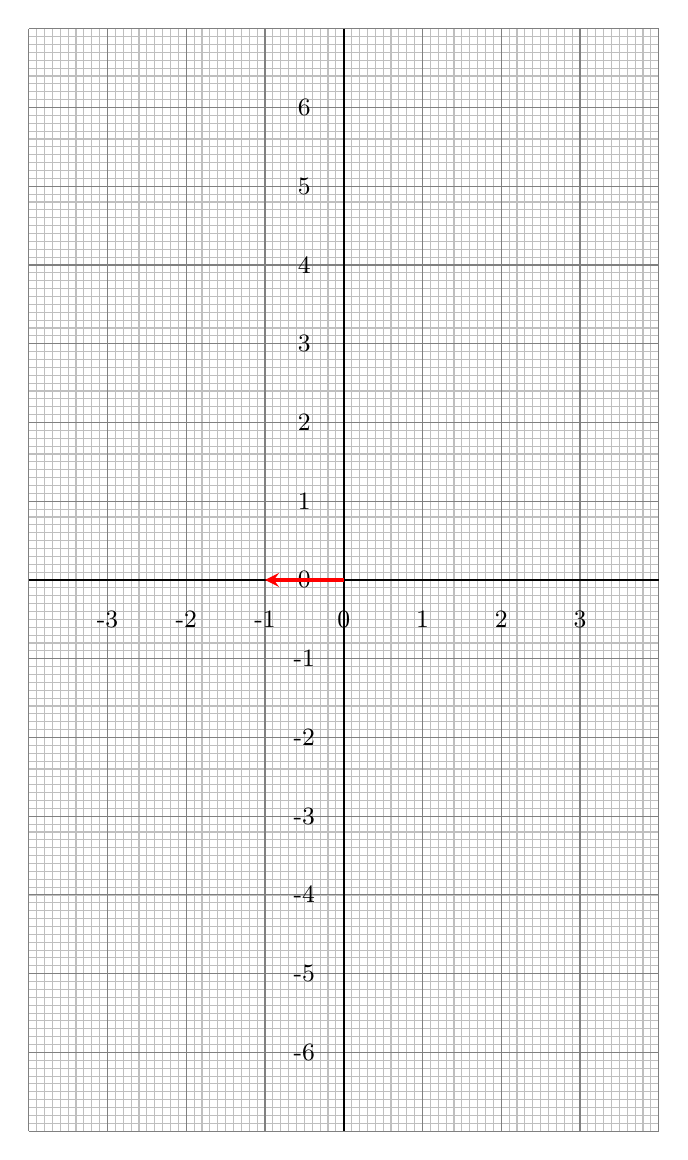
\begin{tikzpicture}
\draw[thin, step=0.1cm,color=lightgray] (-4,-7) grid (4,7);
\draw[thin, step=1cm,color=gray] (-4,-7) grid (4,7);
\draw[thick] (-4,0)--(4,0);
\draw[thick] (0,7)--(0,-7);
\foreach \x in {-3,...,3}{
  \node at (\x,-0.5)  {\small{\x}};
}
\foreach \y in {-6,...,6}{
  \node at (-0.5,\y)  {\small{\y}};
}
\draw [very thick, red, -stealth] (0,0)--(-1,0);
\end{tikzpicture}
&b) 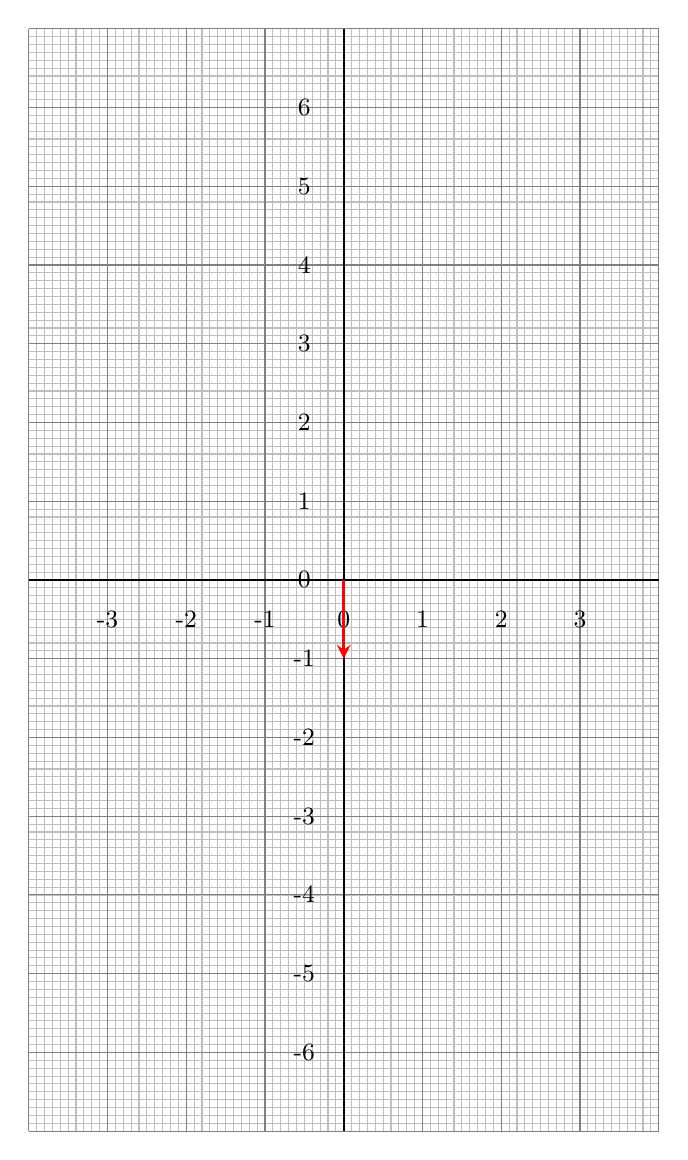
\begin{tikzpicture}
\draw[thin, step=0.1cm,color=lightgray] (-4,-7) grid (4,7);
\draw[thin, step=1cm,color=gray] (-4,-7) grid (4,7);
\draw[thick] (-4,0)--(4,0);
\draw[thick] (0,7)--(0,-7);
\foreach \x in {-3,...,3}{
  \node at (\x,-0.5)  {\small{\x}};
}
\foreach \y in {-6,...,6}{
  \node at (-0.5,\y)  {\small{\y}};
}
\draw [very thick, red, -stealth] (0,0)--(0,-1);
\end{tikzpicture}
\\
\end{tabular}
\newpage
Write in the form $a\mathbf{i}+b\mathbf{j}$:
\newline
\newline
\begin{tabular}{p{9cm}p{9cm}}
a) 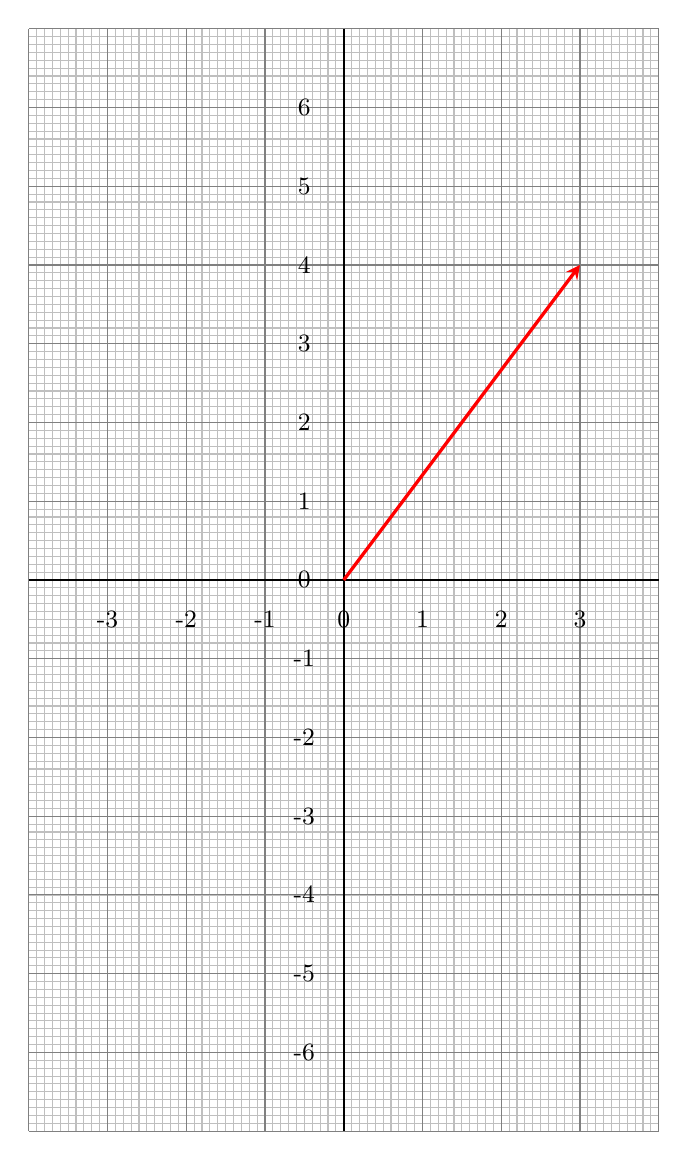
\begin{tikzpicture}
\draw[thin, step=0.1cm,color=lightgray] (-4,-7) grid (4,7);
\draw[thin, step=1cm,color=gray] (-4,-7) grid (4,7);
\draw[thick] (-4,0)--(4,0);
\draw[thick] (0,7)--(0,-7);
\foreach \x in {-3,...,3}{
  \node at (\x,-0.5)  {\small{\x}};
}
\foreach \y in {-6,...,6}{
  \node at (-0.5,\y)  {\small{\y}};
}
\draw [very thick, red, -stealth] (0,0)--(3,4);
\end{tikzpicture}
&b) 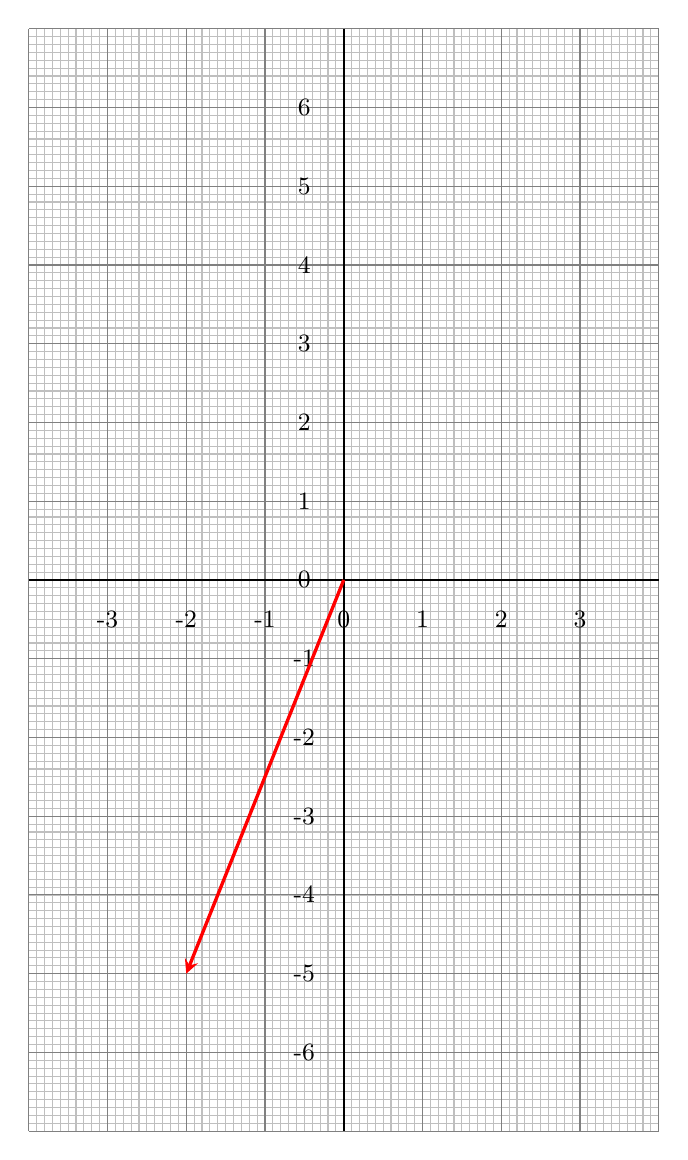
\begin{tikzpicture}
\draw[thin, step=0.1cm,color=lightgray] (-4,-7) grid (4,7);
\draw[thin, step=1cm,color=gray] (-4,-7) grid (4,7);
\draw[thick] (-4,0)--(4,0);
\draw[thick] (0,7)--(0,-7);
\foreach \x in {-3,...,3}{
  \node at (\x,-0.5)  {\small{\x}};
}
\foreach \y in {-6,...,6}{
  \node at (-0.5,\y)  {\small{\y}};
}
\draw [very thick, red, -stealth] (0,0)--(-2,-5);
\end{tikzpicture}
\\
\end{tabular}
\newpage
Write in the form $a\mathbf{i}+b\mathbf{j}$:
\newline
\newline
\begin{tabular}{p{9cm}p{9cm}}
a) 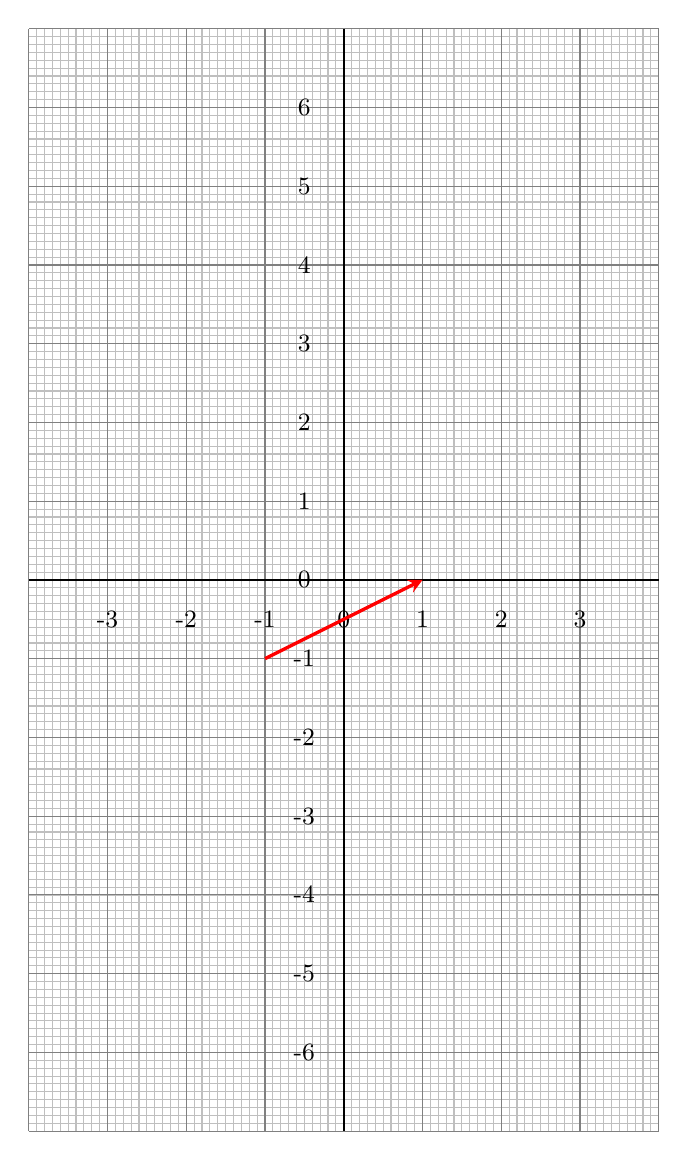
\begin{tikzpicture}
\draw[thin, step=0.1cm,color=lightgray] (-4,-7) grid (4,7);
\draw[thin, step=1cm,color=gray] (-4,-7) grid (4,7);
\draw[thick] (-4,0)--(4,0);
\draw[thick] (0,7)--(0,-7);
\foreach \x in {-3,...,3}{
  \node at (\x,-0.5)  {\small{\x}};
}
\foreach \y in {-6,...,6}{
  \node at (-0.5,\y)  {\small{\y}};
}
\draw [very thick, red, -stealth] (-1,-1)--(1,0);
\end{tikzpicture}
&b) 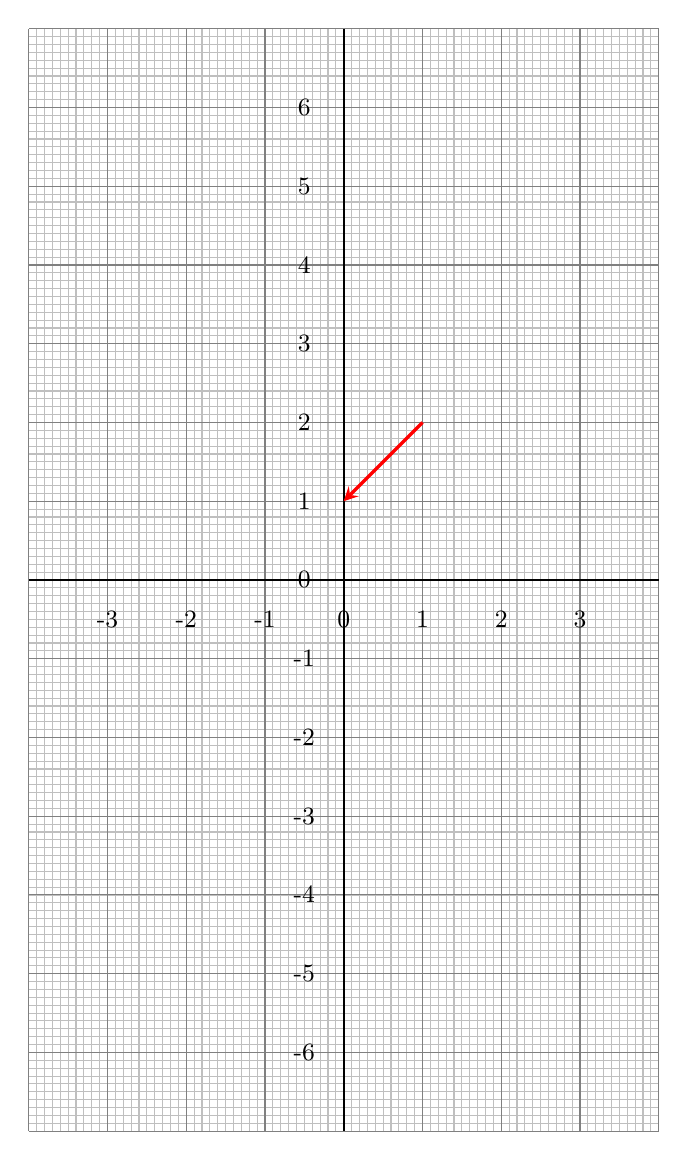
\begin{tikzpicture}
\draw[thin, step=0.1cm,color=lightgray] (-4,-7) grid (4,7);
\draw[thin, step=1cm,color=gray] (-4,-7) grid (4,7);
\draw[thick] (-4,0)--(4,0);
\draw[thick] (0,7)--(0,-7);
\foreach \x in {-3,...,3}{
  \node at (\x,-0.5)  {\small{\x}};
}
\foreach \y in {-6,...,6}{
  \node at (-0.5,\y)  {\small{\y}};
}
\draw [very thick, red, -stealth] (1,2)--(0,1);
\end{tikzpicture}
\\
\end{tabular}
\newpage
Write as column vectors:
\newline
\newline
\begin{tabular}{p{9cm}p{9cm}}
a) $3\mathbf{i}+4\mathbf{j}$
&b) $3\mathbf{i}$
\\\\\\
\\\\\\

c) $-4\mathbf{j}$
&d) $-3\mathbf{i}+\mathbf{j}$
\\\\\\
\\\\\\

e) $3.1234\mathbf{i}$
&f) $-\mathbf{j}$
\\\\\\
\end{tabular}
\newpage
Work out the matrix calculations
\newline
\newline
\begin{tabular}{p{9cm}p{9cm}}
a) $\begin{pmatrix}4\\-2 \end{pmatrix} + \begin{pmatrix}-3\\-1 \end{pmatrix}$
&b) $\begin{pmatrix}14\\-2 \end{pmatrix} - \begin{pmatrix}23\\1 \end{pmatrix}$
\\\\\\
\\\\\\

c) $4\begin{pmatrix}4\\-2 \end{pmatrix} + 2\begin{pmatrix}-3\\-1 \end{pmatrix}$
&d) $-2\begin{pmatrix}14\\-2 \end{pmatrix} - \begin{pmatrix}23\\1 \end{pmatrix}$
\\\\\\
\\\\\\

e) $\begin{pmatrix}1&2\\3&4 \end{pmatrix}+\begin{pmatrix}5&6\\7&8 \end{pmatrix}$
&f) $\begin{pmatrix}1&-2\\3&-4 \end{pmatrix}+\begin{pmatrix}-5&6\\-7&8 \end{pmatrix}$
\\\\\\
\end{tabular}
\newpage
Work out the matrix calculations
\newline
\newline
\begin{tabular}{p{9cm}p{9cm}}
a) $-2\begin{pmatrix}1&2\\3&4 \end{pmatrix}+3\begin{pmatrix}5&6\\7&8 \end{pmatrix}$
&b) $-\begin{pmatrix}1&-2\\3&-4 \end{pmatrix}-\begin{pmatrix}-5&6\\-7&8 \end{pmatrix}$
\\\\\\
\\\\\\

c) $-2\begin{pmatrix}1&2a\\3b&4 \end{pmatrix}+3\begin{pmatrix}5&6c\\7&8 \end{pmatrix}$
&d) $-x\begin{pmatrix}1&-2\\3&-4 \end{pmatrix}-\begin{pmatrix}-5&6\\-7&8 \end{pmatrix}$
\\\\\\
\\\\\\

e) $\begin{pmatrix}1&2\\3&4 \end{pmatrix}\begin{pmatrix}5\\7 \end{pmatrix}$
&f) $\begin{pmatrix}1&-2\\3&-4 \end{pmatrix} \begin{pmatrix}-2\\0 \end{pmatrix}$
\\\\\\
\end{tabular}
\newpage
Work out the matrix calculations
\newline
\newline
\begin{tabular}{p{9cm}p{9cm}}
a) $\begin{pmatrix}1&2\\3&4 \end{pmatrix}\begin{pmatrix}x\\y \end{pmatrix}$
&b) $\begin{pmatrix}1&-2\\3&-4 \end{pmatrix} \begin{pmatrix}-2x+2\\z \end{pmatrix}$
\\\\\\
\\\\\\

c) $\begin{pmatrix}1&2 \end{pmatrix}\begin{pmatrix}3\\4 \end{pmatrix}$
&d) $\begin{pmatrix}1&-2 \end{pmatrix} \begin{pmatrix}-2x\\z \end{pmatrix}$
\\\\\\
\\\\\\

e) $\begin{pmatrix}1&2 \end{pmatrix}\begin{pmatrix}x&4\\y&7 \end{pmatrix}$
&f) $\begin{pmatrix}1&-2 \end{pmatrix} \begin{pmatrix}-2&2\\-15&3 \end{pmatrix}$
\\\\\\
\end{tabular}
\newpage
Work out the matrix calculations
\newline
\newline
\begin{tabular}{p{9cm}p{9cm}}
a) $\begin{pmatrix}1&2\\3&4 \end{pmatrix} \begin{pmatrix}5&6\\7&8 \end{pmatrix}$
&b) $\begin{pmatrix}1&-2\\3&-4 \end{pmatrix} \begin{pmatrix}-5&6\\-7&8 \end{pmatrix}$
\\\\\\

\end{tabular}
\end{document}
